% Document props and library inclusions
\documentclass[t]{beamer} 
\usetheme{%
%Antibes%
%Bergen%
%Berkeley%
%Berlin%
%Copenhagen%
%Darmstadt%
%Dresden%
%Frankfurt%
%Goettingen%
%Hannover%
%Ilmenau%
%JuanLesPins%
%Luebeck%
%Madrid%
%Malmoe%
%Marburg%
Montpellier%
%PaloAlto%
%Pittsburgh%
%Rochester%
%Singapore%
%Szeged%
%Warsaw%
%boxes%
%default%
%CambridgeUS%
}
\usecolortheme{seagull}
\usepackage[utf8]{inputenc} 
\usepackage[swedish]{babel}
\usepackage{mathtools,tikz,textcomp,fixltx2e,color,graphicx,afterpage,float,parskip,xfrac,gensymb,etoolbox}
\usetikzlibrary{calc,matrix,positioning,arrows,shapes,trees,plotmarks,decorations.markings}
\usepackage[font={small,it}]{caption}
\usepackage[europeancurrents,europeanvoltages,europeanresistors,europeaninductors,smartlabels]{circuitikz}
\usepackage[font={small,it}]{caption} %% Italics in captions

\setcounter{secnumdepth}{0} % Levels enumerated
\setcounter{tocdepth}{0} % ToC levels enumerated

\graphicspath{{../designspec/fig/}} % including pictures from here

\title{MatLabb}
\subtitle{Teknisk design}
\author{Matteus Laurent, Johan Levinsson, Oscar Petersson,\\ Erik Peyronson}

\def\swidth{1.8cm}
\setbeamersize{sidebar width left=\swidth}
\setbeamertemplate{sidebar left}
{
  {\usebeamerfont{title in sidebar}%
    \vskip1.5em%
    \usebeamercolor[fg]{title in sidebar}%
    \insertshorttitle[width=\swidth,center,respectlinebreaks]\par%
    \vskip1.25em%
  }%
  {%
    \usebeamercolor[fg]{author in sidebar}%
    \usebeamerfont{author in sidebar}%
    \insertshortauthor[width=\swidth,left,respectlinebreaks]\par%
    \vskip1.25em%
  }%
  \hbox to2cm{\hss\insertlogo\hss}
  \vskip1.25em%
  \insertverticalnavigation{\swidth}%
  \vfill
  \hbox to2cm{\hskip0.6cm\usebeamerfont{subsection in
      sidebar}\strut\usebeamercolor[fg]{subsection in
      sidebar}\insertframenumber/\inserttotalframenumber\hfill}%
  \vskip3pt%
}%

\def\theight{1.8cm}

\setbeamertemplate{headline}
{%
  \begin{beamercolorbox}{section in head/foot}
    \vskip2pt\insertnavigation{\paperwidth}\vskip2pt
  \end{beamercolorbox}%
}

% \setbeamertemplate{frametitle}
%{
%  \nointerlineskip
%  \begin{beamercolorbox}[sep=0.3cm,ht=3em,wd=\paperwidth]{frametitle}
%    \vbox{}\vskip-2ex%
%    \strut\insertframetitle\vskip.8pt\insertframesubtitle\strut
%    \vskip-0.8ex%
%  \end{beamercolorbox}
%}
\beamertemplatenavigationsymbolsempty

%\setbeamerfont{page number in head/foot}{size=\normalsize}
%\setbeamertemplate{footline}[frame number]

\begin{document}
\addtocounter{framenumber}{-1}
\frame{\titlepage}
%Frame 1
%Manus:

% Har du kylen full med matvaror men ingen aning om vad dom skall vara
%bra till?

%Har du svårt att få pengarna att räcka till slutet av månaden och
%behöver hjälp med att dra ner på kostnaderna?

%Försöker du gå ner i vikt men har svårt att hitta kalorisnåla recept?

%Eller kanske är det åt andra hållet och du har svårt att hitta
%energirika?

%Räds icke batlabb är äntligen här!

\begin{frame}
  \frametitle{Matlab}
  \framesubtitle{Inroduktion}
  \begin{itemize}
  \item<1-> Kylen full men ingen inspiration?
  \item<2-> Magen kurrar och kontot tomt?
  \item<3-> Är dieten svår att hålla?
    \begin{itemize}
    \item<4-> Eller går bulken trögt?
    \end{itemize}
  \item<5-> Räds icke, Matlabb är äntligen här!
  \end{itemize}
\end{frame}


%Frame 2 vad är matlabb?
%Manus:
%Matlabb är en interaktiv receptdatabas som hjälper dig organisera
%recept, spara pengar och hålla koll på vad du äter

%Matlab organiserar Recept med Information om tidsåtgång pris
%energiinnehåll, råvaror och beskrivning,

%Det lagrar information om råvarors pris och energiinnehåll vilket gör
%att recepts prisinformation automatiskt uppdateras om ett recept
%ändras.

%Det lagrar information om vilka allergener en ingrediens innehåller
%samt ifall den går bra att ätas av de vanligaste kosthållningarna.

%Och det erbjuder enkelt åtkomst till dina recept med hjälp av
%avancerade filtreringsfunktioner.


\begin{frame}
  \frametitle{Matlab}
  \framesubtitle{Vad är matlabb?}
  \begin{itemize}
  \item<1-> Interaktiv receptdatabas.
  \item<2-> Sparar och organiserar:
    \begin{itemize}
    \item<2-> Recept.
    \item<3-> Råvarors pris och näringsinnehåll.
    \item<4-> Råvarors allergenerer och kosthållning.
    \end{itemize}
  \item<5-> Enkel åtkomst via avancerade sökfilter.
  \end{itemize}
\end{frame}

\begin{frame}
  \frametitle{MatLabb}
  \framesubtitle{Översikt}
  \begin{itemize}
    \item MatLabb har tre delsystem:
      \begin{itemize}
        \item GUI -- Det grafiska användargränssnittet
        \item Shell -- Innehåller objekt och variabler
        \item Lookup -- Verktyg för kommunikation med databasen
      \end{itemize}
  \end{itemize}
\end{frame}

\begin{frame}
  \frametitle{MatLabb}
  \framesubtitle{Klasser och datatyper}
  \begin{itemize}
  \item \textbf{Klasser}
    \begin{itemize}
    \item \texttt{Shell, Recipe, Lookup, (SearchTerm)}
    \item \texttt{InfoIngredient, RecipeIngredient, (Ingredient)}
    \end{itemize}
  \item \textbf{Structs}
    \begin{itemize}
    \item \texttt{MiniRecipe, RelatedRecipe}
    \end{itemize}
  \end{itemize}
\end{frame}

\begin{frame}
  \frametitle{MatLabb}
  \framesubtitle{Klassdiagram}
  \centering
  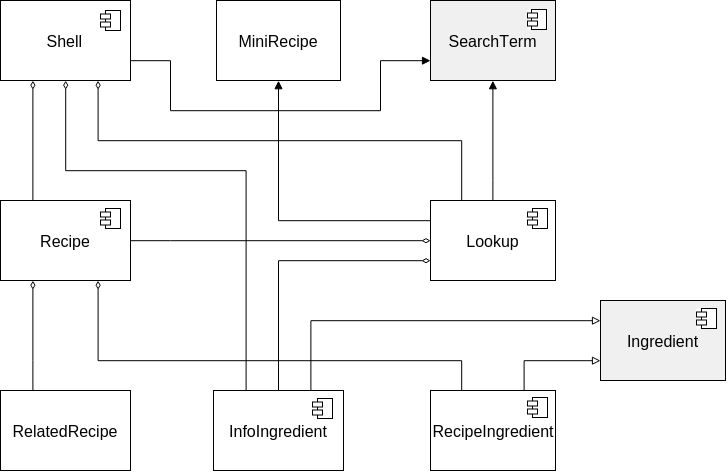
\includegraphics{klass-bantad.png}
\end{frame}

%%%%%%%%%%%%%%%%%%%%%%%%%%%%%%%%%%%%%%%%%%%%%%%%%%%%%%%%%%%%%%%%%%%%%%%%%%%%%%%%%%%%%%%%%%
% Dokumenttypen Beamer låter oss skapa slides m.h.a. LaTeX
%
% I stort sett allt fungerar som ni är vana vid när det kommer till  formatering, men
% en markant skillnad är \verb som inte fungerar.  Använd i stället
% \texttt{<insert text here>}.
%
% Ny slide sätts i miljön ``frame''. Se gärna dummies och sliden i TSIU03 för basic stuff.
% Full dokumentation återfinns på:
% http://ftp.acc.umu.se/mirror/CTAN/macros/latex/contrib/beamer/doc/beameruserguide.pdf
%%%%%%%%%%%%%%%%%%%%%%%%%%%%%%%%%%%%%%%%%%%%%%%%%%%%%%%%%%%%%%%%%%%%%%%%%%%%%%%%%%%%%%%%%%

\begin{frame}
  \frametitle{foo}
  \begin{block}{Meep}
    Burp!
  \end{block}
\end{frame}

%%%%%%%%%%%%%%%%%%%%%%%%%%%%%%%%%%%%%%%%%%%%%%%%%%%%%%%%%%%%%%%%%%%%%%%%%%%%%%%%%%%%%%%%%%%
% Dokumenttypen Beamer låter oss skapa slides m.h.a. LaTeX
%
% I stort sett allt fungerar som ni är vana vid när det kommer till  formatering, men
% en markant skillnad är \verb som inte fungerar.  Använd i stället
% \texttt{<insert text here>}.
%
% Ny slide sätts i miljön ``frame''. Se gärna dummies och sliden i TSIU03 för basic stuff.
% Full dokumentation återfinns på:
% http://ftp.acc.umu.se/mirror/CTAN/macros/latex/contrib/beamer/doc/beameruserguide.pdf
%%%%%%%%%%%%%%%%%%%%%%%%%%%%%%%%%%%%%%%%%%%%%%%%%%%%%%%%%%%%%%%%%%%%%%%%%%%%%%%%%%%%%%%%%%

\begin{frame}
  \frametitle{foo}
  \begin{block}{Meep}
    Burp!
  \end{block}
\end{frame}

%\begin{figure}[h]
  \centering
  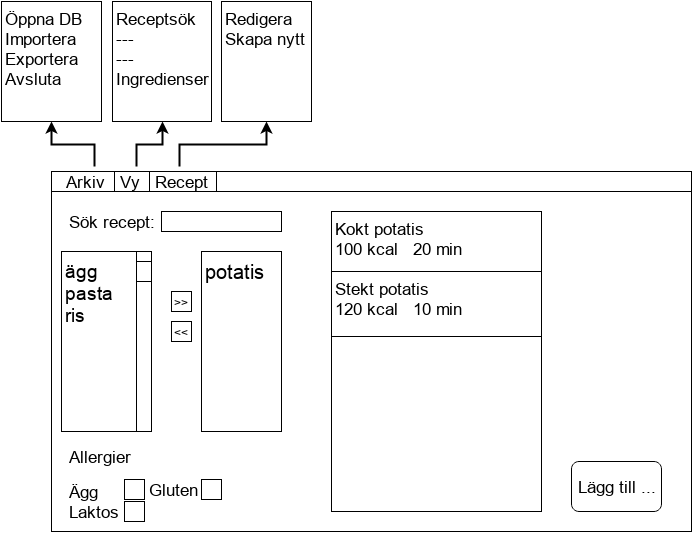
\includegraphics[scale=.5]{vy1.png}
  \label{fig:vy1}
  \caption{Sökfönster}
\end{figure}

\begin{figure}[h]
  \centering
  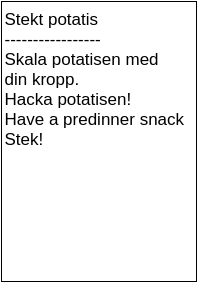
\includegraphics[scale=.5]{vy2.png}
  \label{fig:vy2}
  \caption{Receptfönster}
\end{figure}

\begin{figure}[h]
  \centering
  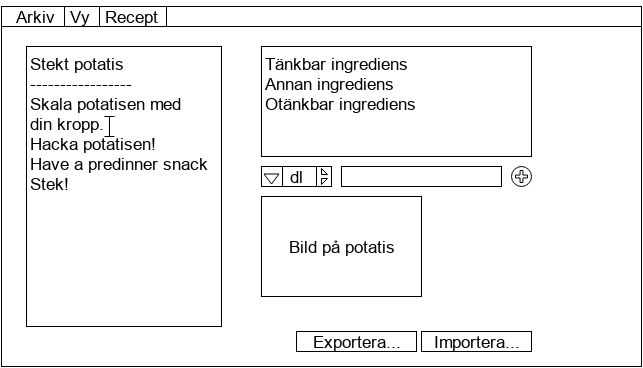
\includegraphics[scale=.5]{vy3.png}
  \label{fig:vy3}
  \caption{Redigering av recept}
\end{figure}

\begin{figure}[h]
  \centering
  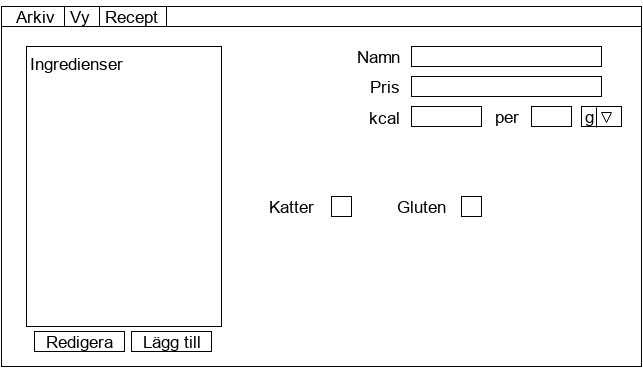
\includegraphics[scale=.5]{vy4.png}
  \label{fig:vy4}
  \caption{Redigering av ingredienser}
\end{figure}

Då all receptinforamtion behöver sparas mellan körningar av programmet
behöver den lagras externy. I det här programmet kommer en databas
användas med hjälp av MySQL. Databasen kan överskådas i
EER-diagramet i \ref{fig:erdiagram}. Den del som ligger innom de streckade området hör
till funktionalitet som endast kommer implementeras i mån av tid.

\begin{figure}[H]
        \centering
        \includegraphics[scale=0.35]{erdiagram.png}
        \caption{Entity-Relationship diagram}
        \label{fig:erdiagram}
\end{figure}

Databasen kommer bestå av fem entiteter \verb+Recipe+ som innehåller
information unik för ett enskilt recept. \verb+Ingredient+ som är en lista
över de olika ingredienser som databasen innehåller, \verb+Allergy+
som är en lista över allergier, \verb+Tool+ som är en lista över allergier samt
\verb+Comment+ som är en lista över kommentarer till varje recept.

Entiteten \verb+Recipe+ är den entiteten som lagrar namn, beskrivning, bild
tillagningsmetod, då recept skall ha unika namn för att särskilja dem åt är det
receptets namn som agerar primärnyckel.

\verb+Recipe+ har en m-n relation till \verb+Ingredient+ vilket ger oss en
lista på ingredienser till vajre recept. Genom att ha attributen \verb+kcal+ och \verb+price+
på entiteten \verb+Ingredients+ istället för \verb+Recipe+ behöver unik information om
portionspris och närings-inehåll till varje recept inte sparas utan kan räknas ut beroende på vilka
ingredienser som ingår. Genom att tillföra attributet \verb+amount+ behöver varje ingrediens
endast lagras en gång per recept och enhetsomvandling och portionsskalning kommer vara möjlig.

För att hålla ordning på de vanligaste matallergierna (samt kött mejeri och fisk för
veganer/veganer) finns entiteten \verb+Allergy+. Den har även en 1-n relation till \verb+Comment+
vilket resulterar i att alla recept får en lista med komentarer skrivna av användaren. samt en
m-n relation till \verb+Tool+ som ger en lista över de redskaps som behövs.

Genom att utforma databasen enligt sagda modell kommer programmet kunna utföra sökningar olika
sökningar och filtreringar på ingredienser som ingår, inte ingår, eventuella allergener etc.






\end{document}
